
\begin{figure}[h!]

  \centering    
    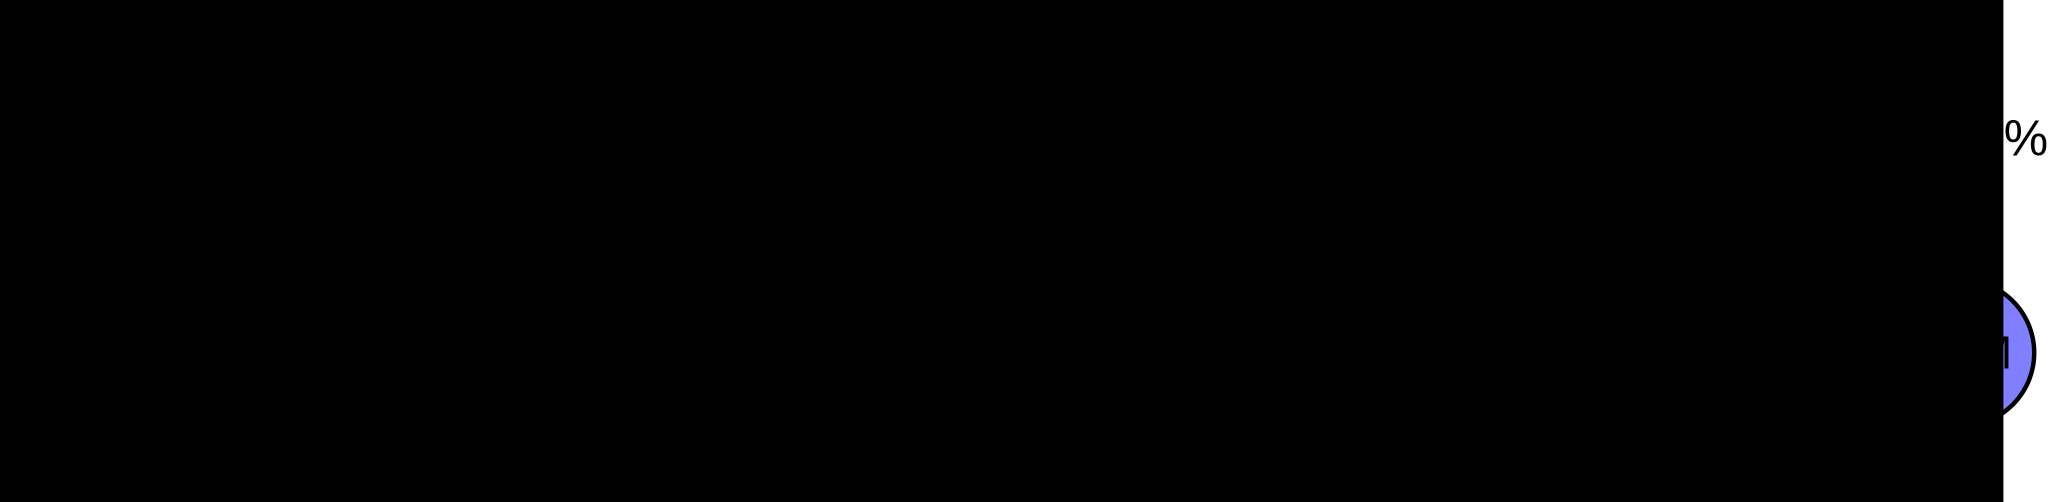
\includegraphics[width=0.95\textwidth]{figures/sleep_description.pdf}
  \caption{\ctit{Structural description of sleep stages.}
  \textbf{A}: Characteristics of the three sleep stages.
  Typically, frequency and amplitude of the \acrfull{eeg}, and amplitude of the \acrfull{emg} are used by experts to infer sleep stage.
  The presented frequency ranges and and pevalences are approximate values for healthy adult animals in normal conditions.
  Each wave shows a representative five second epoch with high signal to noise ratio.
  \textbf{B}: Empirical transition probabilities between consecutive five second epochs. The width of the arrow is proportionnal to the probability of transition.
  Probabilities of remaining in the three state are implied.
  \label{fig:sleep_description}
  }
           
\end{figure}
